\documentclass[10pt]{article}
\usepackage[utf8]{inputenc}

\title{Introdução à Multimídaia}
\author{ajs7@cin.ufpe.br }
\date{05/11/2019}

\usepackage{natbib}
\usepackage{graphicx}

\begin{document}

\maketitle

\section{Introdução à Multimídia}
A disciplina de Introdução à Multimídia se originou através de uma necessidade e dos interesses entre o corpo doscente e discente da UFPE, em criar ambientes virtuais e aplicações de multimídia.
O curso é oferecido para alunos nos níveis de graduação(IF687) e pós-graduação(IF124).
Durante a graduação o curso da ênfase na implementação de ambientes virtuais, já na pós-graduação o curso da ênfase ao suporte de uso inteligente de mundos virtuais como um suporte para aplicações multimídia.

\begin{figure}[!htb]
    \centering
    \caption{Imagem ilustrativa 1.}
    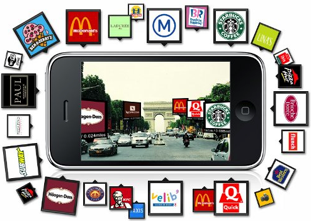
\includegraphics[scale=1]{imagens/figura.png}\\
    {\footnotesize Fonte: https://www.cin.ufpe.br/~if687/imagens/fig5.png}
    \label{fig:my_label}
\end{figure}

\section{Objetivos do Curso}
Um dos objetivos dessa disciplina é apresentar os conceitos básicos, definições e ferramentas para multimídia. Dando um foco operacional.
Especificando: Desenvolver a capacidade de criar mundos virtuais, com ênfase na internet, como foco em visualização de dados, aplicações em educação, medicina, entretenimento, etc.
Desenvolver a capacidade de especificar construir e avaliar componentes multimídia específicos para esses mundos virtuais.

\section{Relevância}
Essa disciplina é bastante relevânte pois agrega um dos temas mais utilizados no mundo, o conteúdo relacionado a multimídia, que atualmente é um dos mercados mais rentáveis no mundo tecnológico.

\begin{figure}[!htb]
    \centering
    \caption{Imagem ilustrativa 2.}
    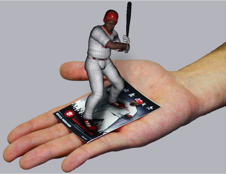
\includegraphics[scale=1]{imagens/fig3.png}\\
    {\footnotesize Fonte:https://www.cin.ufpe.br/~if687/imagens/fig3.png}
    \label{fig:my_label}
\end{figure}



\bibliographystyle{plain}
\cite{Judith}
\bibliography{ajs7}
\end{document}
